% !TeX root = ../thesis.tex
\chapter{THIẾT KẾ VÀ THỰC HIỆN PHẦN MỀM}

\section{Kiến trúc phần mềm ROS 2}

\subsection{Tổng quan kiến trúc node}

Hệ thống phần mềm được triển khai trên nền tảng ROS~2 Humble \cite{ros2docs}, sử dụng kiến trúc xử lý phân tán gồm hai node tính toán được phân vùng theo chức năng:

\begin{itemize}
    \item \textbf{Gait Generator Node:} Quản lý toàn bộ quá trình tính toán quỹ đạo tuần hoàn, giải bài toán động học nghịch và gửi lệnh điều khiển đến các cơ cấu chấp hành qua bus nối tiếp. Node này được lập trình bằng Python, bao gồm các module: \texttt{gaitGenerator.py} (37KB -- tạo dáng đi), \texttt{kinematics.py} (IK solver), \texttt{quinticPlanning.py} (nội suy đa thức bậc 5) và \texttt{serialPublish.py} (giao tiếp UART với servo).
    
    \item \textbf{Balance Controller Node:} Xử lý bất đồng bộ việc thu thập dữ liệu quán tính tần số cao, xử lý tín hiệu đa giai đoạn và tính toán bù PID. Node này hoạt động độc lập qua module \texttt{nodeBalanceController.py} (22KB).
\end{itemize}

\subsection{Giao tiếp giữa các node}

Giao tiếp liên tiến trình giữa hai node sử dụng cơ chế publish-subscribe qua DDS (Data Distribution Service) của ROS~2. Balance Controller node phát các thông điệp vector hiệu chỉnh nhẹ trên các topic bất đồng bộ chuyên dụng. Kiến trúc tách rời này đảm bảo rằng các nút thắt xử lý tại Gait Generator không thể chiếm quyền hoặc chặn các bù trừ cảm biến quan trọng, cho phép vận hành xác định, chịu lỗi ngay cả dưới tải CPU cao.

Sơ đồ tổng thể kiến trúc ROS~2 bao gồm các node, topic và luồng dữ liệu giữa các thành phần được thể hiện trong Hình~\ref{fig:ros2_arch}. Sơ đồ phân biệt rõ các thành phần theo loại: ROS~2 node (Python), driver (C++), topic truyền thông, cảm biến phần cứng, và giao diện mô phỏng Gazebo.

\begin{figure}[H]
    \centering
    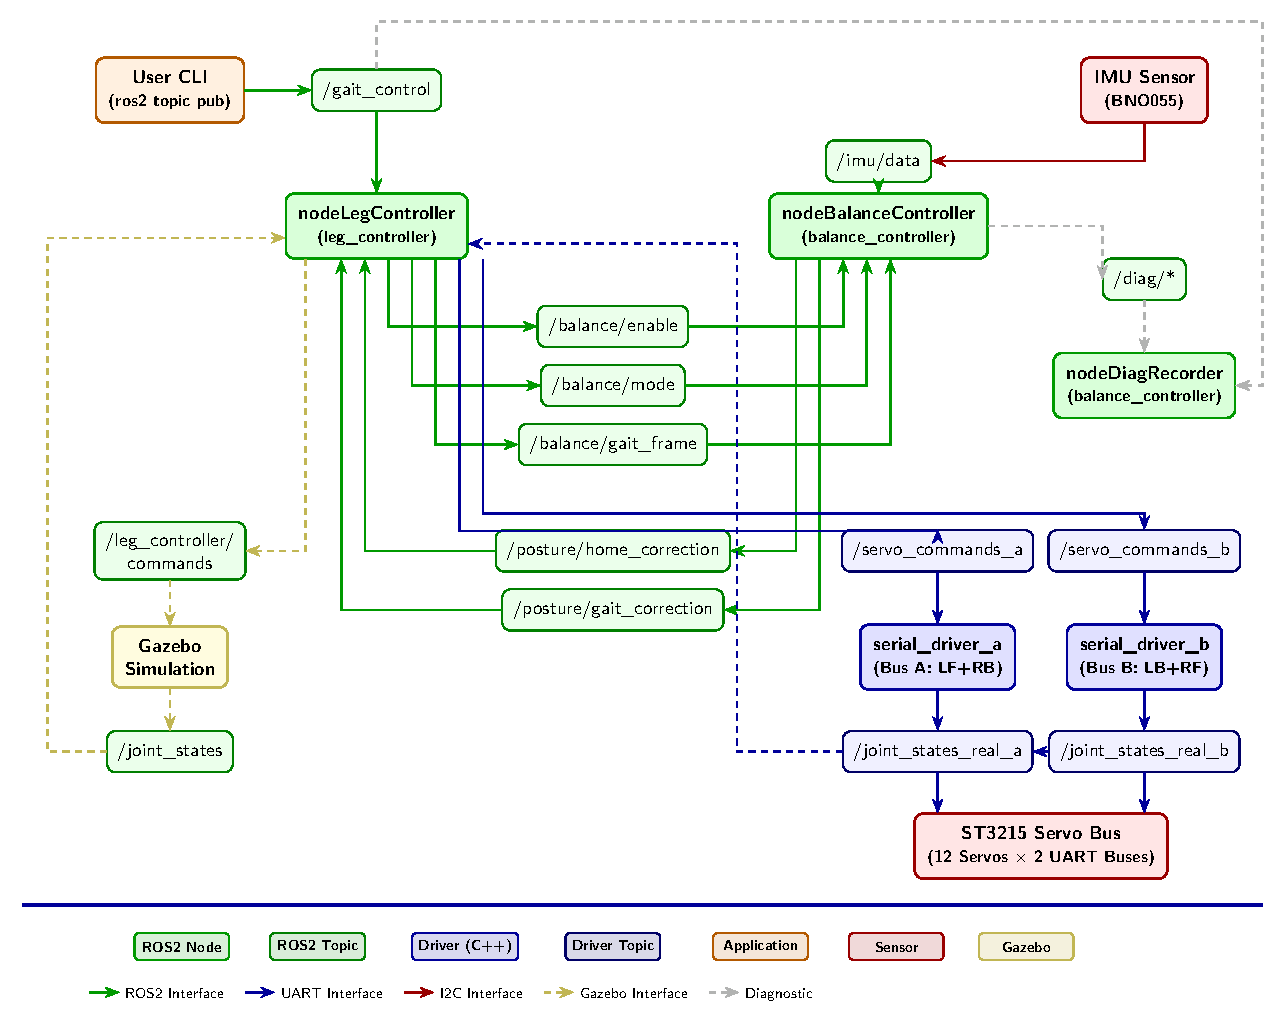
\includegraphics[width=\textwidth]{img/fig_ros2_architecture.pdf}
    \caption{Sơ đồ kiến trúc ROS~2 của hệ thống: các node, topic và luồng dữ liệu}
    \label{fig:ros2_arch}
\end{figure}

\subsection{Các trạng thái vận hành}

Hệ thống quản lý hai trạng thái vận hành rời rạc thông qua cổng logic boolean:

\begin{itemize}
    \item \textbf{HOME:} Cấu hình tĩnh không có vector tịnh tiến tuần hoàn. Bộ điều khiển tính toán các điều chỉnh đồng nhất trong không gian khớp, ánh xạ cứng đến tư thế nghỉ. Sai lệch góc cơ sở được chuyển đổi tỷ lệ thành các bù mô-men đối kháng nhằm hiệu chỉnh tư thế liên tục. Một khoảng trễ khởi động $T_{delay}$ giây có thể cấu hình giúp ngăn hiệu chỉnh sớm trong giai đoạn quá độ khởi tạo hệ thống.
    
    \item \textbf{GAIT:} Trạng thái động kích hoạt khi có lệnh tịnh tiến mặt phẳng. Robot thực hiện quỹ đạo đa thức tuần hoàn sử dụng các mảng dịch pha khả cấu hình để tạo dáng đi trot ($\phi = [0, 0, 0{,}5, 0{,}5]$), walk ($\phi = [0, 0{,}25, 0{,}5, 0{,}75]$) và các dáng đi khác. Các hiệu chỉnh không gian từ phản hồi quán tính chỉ được áp dụng cho chân ở pha chống, trong khi chân ở pha bay duy trì bù bằng không để đảm bảo khoảng trống sải bước.
\end{itemize}

\subsection{Cấu trúc các ROS 2 packages}

Toàn bộ hệ thống phần mềm được tổ chức thành 6 packages ROS~2:

\begin{table}[H]
\centering
\caption{Cấu trúc các ROS 2 packages trong hệ thống}
\label{tab:ros2_packages}
\renewcommand{\arraystretch}{1.3}
\begin{tabular}{|p{0.22\linewidth}|p{0.12\linewidth}|p{0.52\linewidth}|}
\hline
\textbf{Package} & \textbf{Ngôn ngữ} & \textbf{Chức năng} \\ \hline
\texttt{leg\_controller} & Python & Tạo dáng đi, IK solver, quy hoạch quỹ đạo, giao tiếp servo \\ \hline
\texttt{balance\_controller} & Python & Thu thập IMU, xử lý tín hiệu, PID cân bằng, chẩn đoán \\ \hline
\texttt{serial\_driver} & C++ & Driver giao tiếp với bus servo ST3215 (thư viện SCServo) \\ \hline
\texttt{simulation} & Python & Mô hình URDF, cấu hình Gazebo, RViz, launch mô phỏng \\ \hline
\texttt{launch\_main} & CMake & Launch files cho hệ thống thực \\ \hline
\end{tabular}
\end{table}

\subsection{Chi tiết các module phần mềm}

\textbf{Module gaitGenerator.py} là module cốt lõi của hệ thống, quản lý máy trạng thái (state machine) điều khiển toàn bộ vòng đời vận hành của robot. Module này thực hiện các chức năng:

\begin{itemize}
    \item \textbf{Quản lý trạng thái:} Robot chuyển đổi giữa các trạng thái: INIT (khởi tạo) $\rightarrow$ ZERO (homing về tư thế đứng) $\rightarrow$ TROT/WALK/PUSHUP/SWAY (dáng đi) $\rightarrow$ ROBOTOFF (tắt an toàn). Mỗi trạng thái có hàm \texttt{control\_tick()} riêng biệt xử lý một frame điều khiển.
    \item \textbf{Tạo quỹ đạo:} Gọi hàm \texttt{quintic\_planning()} để tạo quỹ đạo hình chữ D cho mỗi chân, sau đó giải IK qua module \texttt{kinematics.py} để chuyển đổi từ tọa độ Đề-các sang góc khớp.
    \item \textbf{Áp dụng hiệu chỉnh IMU:} Nhận tín hiệu bù từ Balance Controller qua hai topic \texttt{/posture/home\_correction} và \texttt{/posture/gait\_correction}, áp dụng vào góc khớp (HOME) hoặc tọa độ bàn chân (GAIT).
    \item \textbf{Xuất lệnh servo:} Gửi góc điều khiển đến module \texttt{serialPublish.py} để chuyển đổi từ góc IK sang góc servo và truyền qua UART.
\end{itemize}

\textbf{Module serialPublish.py} đảm nhận việc chuyển đổi giữa hai chế độ vận hành (mô phỏng và phần cứng thực) thông qua biến cấu hình \texttt{use\_real}:

\begin{itemize}
    \item \textbf{Chế độ mô phỏng:} Xuất bản lệnh mô-men (effort) lên topic \texttt{/effort\_controller/commands} để điều khiển robot trong Gazebo thông qua plugin \texttt{gazebo\_ros2\_control}.
    \item \textbf{Chế độ phần cứng:} Chuyển đổi góc IK sang góc servo bằng các hàm ánh xạ riêng biệt cho từng chân (\texttt{\_ik\_to\_servo\_lf()}, \texttt{\_ik\_to\_servo\_rf()}, v.v.), sau đó xuất bản lên hai topic \texttt{/servo\_commands\_a} và \texttt{/servo\_commands\_b}.
\end{itemize}

\subsection{Bảng giao tiếp topic ROS~2}

Bảng~\ref{tab:ros2_topics} liệt kê các topic chính trong hệ thống, phân loại theo chức năng.

\begin{table}[H]
\centering
\caption{Các topic ROS~2 chính trong hệ thống}
\label{tab:ros2_topics}
\renewcommand{\arraystretch}{1.3}
\begin{tabular}{|p{0.32\linewidth}|p{0.12\linewidth}|p{0.42\linewidth}|}
\hline
\textbf{Topic} & \textbf{Kiểu dữ liệu} & \textbf{Mô tả} \\ \hline
\texttt{/imu/data} & Imu & Dữ liệu quaternion từ BNO055 \\ \hline
\texttt{/balance/enable} & Bool & Bật/tắt bộ PID cân bằng \\ \hline
\texttt{/balance/mode} & String & Chuyển chế độ HOME/GAIT \\ \hline
\texttt{/balance/gait\_frame} & Int32 & Chỉ số frame dáng đi hiện tại \\ \hline
\texttt{/posture/home\_correction} & Vector3 & Tín hiệu bù PID chế độ HOME \\ \hline
\texttt{/posture/gait\_correction} & Vector3 & Tín hiệu bù PID chế độ GAIT \\ \hline
\texttt{/posture/measurement} & Vector3 & Góc roll/pitch đã lọc \\ \hline
\texttt{/servo\_commands\_a} & Float64[] & Lệnh góc cho Driver A (6 servo) \\ \hline
\texttt{/servo\_commands\_b} & Float64[] & Lệnh góc cho Driver B (6 servo) \\ \hline
\end{tabular}
\end{table}

\subsection{Cơ chế chẩn đoán thời gian thực}

Hệ thống tích hợp cơ chế chẩn đoán (diagnostics) cho phép giám sát trực tiếp các biến nội bộ của bộ điều khiển PID trong thời gian thực thông qua công cụ PlotJuggler. Mỗi giai đoạn trong pipeline PID (đo lường $\rightarrow$ sai lệch $\rightarrow$ P/I/D $\rightarrow$ bão hòa $\rightarrow$ lọc) đều có topic chẩn đoán riêng, cho phép:

\begin{itemize}
    \item Quan sát trực tiếp từng thành phần P, I, D và tổng PID
    \item Phát hiện hiện tượng windup hoặc bão hòa đầu ra
    \item So sánh tín hiệu đo (measurement) với điểm đặt (setpoint) để đánh giá chất lượng bám
    \item Ghi lại dữ liệu dưới dạng file CSV để phân tích offline
\end{itemize}

Tổng cộng, hệ thống xuất bản 22 topic chẩn đoán cho chế độ HOME (9 tín hiệu $\times$ 2 trục + 4 tín hiệu áp dụng) và 18 topic cho chế độ GAIT (9 tín hiệu $\times$ 2 trục), cung cấp khả năng quan sát toàn diện đường ống điều khiển.

\section{Quy trình Homing và Calibrate}

\subsection{Calibrate servo}

Trước khi vận hành, mỗi servo cần được calibrate để đảm bảo góc $0^\circ$ cơ học trùng với góc $0^\circ$ trong phần mềm. Quy trình calibrate bao gồm:

\begin{enumerate}
    \item Đặt tất cả chân robot ở tư thế tham chiếu (chân duỗi thẳng, vuông góc với thân).
    \item Đọc vị trí feedback của từng servo qua thư viện SCServo SDK.
    \item Ghi giá trị offset ($\Delta_{calib}$) --- sai lệch giữa vị trí thực tế và vị trí lý thuyết tại góc $0^\circ$.
    \item Lưu offset vào mảng cấu hình trong \texttt{serialPublish.py}, áp dụng tự động trong các lần khởi chạy tiếp theo.
\end{enumerate}

\subsection{Quy trình Homing}

Quy trình homing (đưa robot về tư thế đứng chuẩn) được thực hiện tự động mỗi khi robot khởi động:

\begin{enumerate}
    \item \textbf{Đọc vị trí hiện tại:} Lấy giá trị góc feedback từ tất cả 12 servo ($\theta_{current,i}$).
    \item \textbf{Tính tư thế đích:} Giải IK cho tư thế đứng chuẩn, tạo ra bộ góc đích $\theta_{target,i} = (0^\circ, 0^\circ, 90^\circ)$ cho mỗi chân.
    \item \textbf{Nội suy tuyến tính:} Trong $N_{homing} = 200$ frame, mỗi góc được nội suy tuyến tính:
    \begin{equation}
        \theta_i(k) = \theta_{current,i} + \frac{k}{N_{homing}} (\theta_{target,i} - \theta_{current,i}), \quad k = 0, 1, \ldots, N_{homing}
    \end{equation}
    \item \textbf{Gửi lệnh:} Tại mỗi frame, gửi bộ 12 góc đã nội suy đến servo qua UART.
\end{enumerate}

Phương pháp nội suy tuyến tính đảm bảo chuyển động mượt mà từ bất kỳ vị trí khởi đầu nào, tránh hiện tượng giật hoặc va đập. Tổng thời gian homing: $200 \times 7 = 1400$ ms $\approx 1{,}4$ giây.

